\documentclass[a4paper,11pt]{article}

\usepackage[margin=1in]{geometry}
\usepackage[T1]{fontenc}
\usepackage[utf8]{inputenc}
\usepackage{booktabs}
\usepackage{tabularx}
\usepackage{array}
\usepackage{tikz}
\usepackage[american]{circuitikz}
\usetikzlibrary{arrows.meta, calc, fit, positioning}

\title{6-DOF Robotic Arm\\Electrical Schematic and Wiring Notes}
\author{robotic-arm-control}
\date{\today}

\begin{document}

\maketitle

\section{Overview}

This document summarizes the main electrical wiring for the Arduino Uno based
6-DOF robotic arm controller used in this repository. The design is based on
the current project sources in \texttt{README.md}, \texttt{docs/hardware.md},
and \texttt{diagram.json}.

The system combines:

\begin{itemize}
  \item one Arduino Uno as the main controller,
  \item one Wii Nunchuck connected over I2C,
  \item six servo outputs for the robotic arm joints,
  \item one external \SI{5}{V} to \SI{6}{V} supply dedicated to the servos.
\end{itemize}

All grounds must be tied together. The servo bank must \textbf{not} be powered
from the Arduino \SI{5}{V} pin.

\section{High-Level Architecture}

\begin{figure}[htbp]
\centering
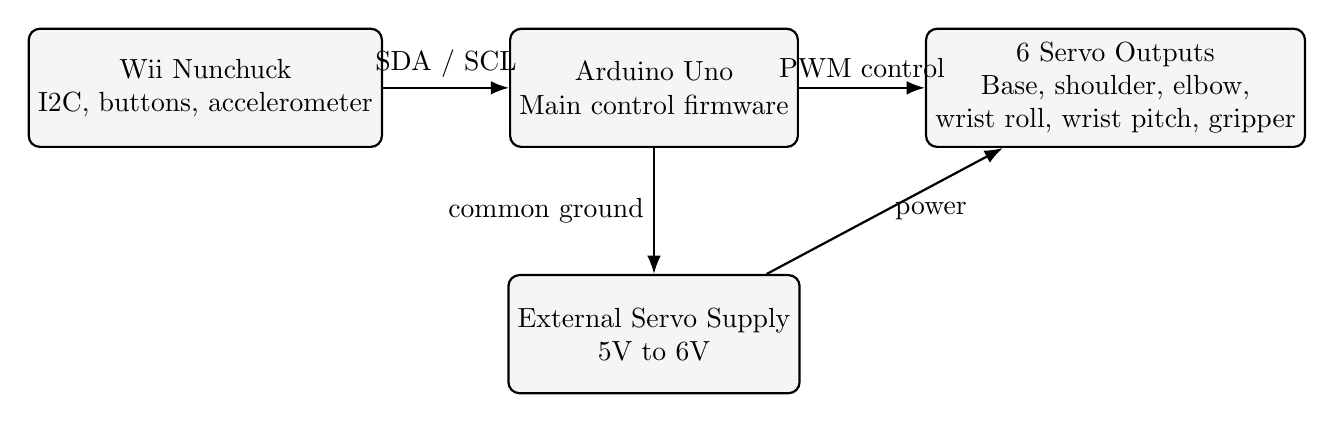
\begin{tikzpicture}[
  node distance=16mm and 16mm,
  block/.style={
    draw,
    rounded corners,
    thick,
    minimum width=3.5cm,
    minimum height=1.5cm,
    align=center,
    fill=gray!8
  },
  arrow/.style={-Latex, thick}
]
  \node[block] (nunchuck) {Wii Nunchuck\\I2C, buttons, accelerometer};
  \node[block, right=of nunchuck] (arduino) {Arduino Uno\\Main control firmware};
  \node[block, right=of arduino] (servos) {6 Servo Outputs\\Base, shoulder, elbow,\\wrist roll, wrist pitch, gripper};
  \node[block, below=of arduino] (supply) {External Servo Supply\\\SI{5}{V} to \SI{6}{V}};

  \draw[arrow] (nunchuck) -- node[above]{SDA / SCL} (arduino);
  \draw[arrow] (arduino) -- node[above]{PWM control} (servos);
  \draw[arrow] (supply) -- node[right]{power} (servos);
  \draw[arrow] (arduino) -- node[left]{common ground} (supply);
\end{tikzpicture}
\caption{High-level control and power architecture.}
\end{figure}

\section{Pin Mapping}

\begin{center}
\begin{tabularx}{\textwidth}{>{\ttfamily}l >{\ttfamily}l X}
\toprule
Signal / Joint & Arduino Pin & Notes \\
\midrule
Base & D3 & Continuous rotation servo, 90 is stop \\
Shoulder & D5 & Positional servo \\
Elbow & D6 & Positional servo \\
Wrist roll & D9 & Positional servo \\
Wrist pitch & D10 & Positional servo \\
Gripper & D11 & Positional servo \\
Nunchuck SDA & A4 & I2C data line \\
Nunchuck SCL & A5 & I2C clock line \\
Nunchuck VCC & 3.3V & Fixed project wiring \\
Common ground & GND & Shared by Arduino, servos, supply, and Nunchuck \\
\bottomrule
\end{tabularx}
\end{center}

\section{Electrical Schematic}

\begin{figure}[p]
\centering
\begin{circuitikz}[x=1cm, y=1cm, every node/.style={font=\small}]
  % Main blocks
  \node[draw, rounded corners, thick, minimum width=4.7cm, minimum height=6.5cm, align=left, fill=blue!5] (uno) at (0,0) {
    \textbf{Arduino Uno}\\[2mm]
    D3  \hspace{7mm} Base servo signal\\
    D5  \hspace{7mm} Shoulder servo signal\\
    D6  \hspace{7mm} Elbow servo signal\\
    D9  \hspace{7mm} Wrist roll signal\\
    D10 \hspace{4mm} Wrist pitch signal\\
    D11 \hspace{4mm} Gripper signal\\[1mm]
    A4  \hspace{7mm} SDA\\
    A5  \hspace{7mm} SCL\\
    3.3V \hspace{7mm} Nunchuck VCC\\
    GND \hspace{6mm} Common ground
  };

  \node[draw, rounded corners, thick, minimum width=3.8cm, minimum height=2.2cm, align=left, fill=green!5] (nunchuck) at (-5.7,2.0) {
    \textbf{Wii Nunchuck}\\[1mm]
    VCC\\
    GND\\
    SDA\\
    SCL
  };

  \node[draw, rounded corners, thick, minimum width=4.2cm, minimum height=2.2cm, align=center, fill=red!5] (psu) at (-5.7,-3.2) {
    \textbf{External Servo Supply}\\
    \SI{5}{V} to \SI{6}{V}
  };

  % Servo nodes
  \node[draw, rounded corners, thick, minimum width=3.8cm, minimum height=0.9cm, align=left, fill=yellow!8] (servo1) at (7.2,3.0) {Base servo \hfill D3};
  \node[draw, rounded corners, thick, minimum width=3.8cm, minimum height=0.9cm, align=left, fill=yellow!8] (servo2) at (7.2,1.9) {Shoulder servo \hfill D5};
  \node[draw, rounded corners, thick, minimum width=3.8cm, minimum height=0.9cm, align=left, fill=yellow!8] (servo3) at (7.2,0.8) {Elbow servo \hfill D6};
  \node[draw, rounded corners, thick, minimum width=3.8cm, minimum height=0.9cm, align=left, fill=yellow!8] (servo4) at (7.2,-0.3) {Wrist roll \hfill D9};
  \node[draw, rounded corners, thick, minimum width=3.8cm, minimum height=0.9cm, align=left, fill=yellow!8] (servo5) at (7.2,-1.4) {Wrist pitch \hfill D10};
  \node[draw, rounded corners, thick, minimum width=3.8cm, minimum height=0.9cm, align=left, fill=yellow!8] (servo6) at (7.2,-2.5) {Gripper \hfill D11};

  \node[draw, dashed, inner sep=0.35cm, fit=(servo1)(servo2)(servo3)(servo4)(servo5)(servo6), label=above:{Servo bank}] {};

  % Power bus and ground bus
  \draw[very thick, red!75!black] (-3.8,-1.3) -- (9.6,-1.3);
  \node[anchor=west] at (9.65,-1.3) {Servo V+ bus};

  \draw[very thick] (-6.9,-4.9) -- (9.6,-4.9);
  \node[anchor=west] at (9.65,-4.9) {Common GND};

  % PSU to buses
  \draw[very thick, red!75!black] (psu.east) -- ++(1.2,0) |- (-3.8,-1.3);
  \draw[very thick] (psu.south) -- ++(0,-1.0) |- (-6.2,-4.9);

  % Arduino to common ground
  \draw[thick] ($(uno.south west)+(1.0,0)$) -- ++(0,-1.7) |- (0.0,-4.9);
  \node[below] at (0.0,-4.9) {};

  % Nunchuck power and I2C
  \draw[orange!80!black, dashed, thick] ($(uno.west)+(0,0.6)$) -- ++(-0.8,0) |- (nunchuck.south);
  \node[orange!80!black, align=center] at (-3.8,0.2) {VCC\\3.3V};

  \draw[thick] ($(nunchuck.south west)+(0.9,0)$) -- ++(0,-0.9) |- (-4.6,-4.9);

  \draw[blue!70!black, thick] ($(uno.west)+(0,1.7)$) -- ++(-1.0,0) |- ($(nunchuck.east)+(0,-0.35)$);
  \draw[blue!70!black, thick] ($(uno.west)+(0,1.2)$) -- ++(-1.4,0) |- ($(nunchuck.east)+(0,0.35)$);
  \node[blue!70!black, fill=white, inner sep=1pt] at (-2.2,2.2) {SDA};
  \node[blue!70!black, fill=white, inner sep=1pt] at (-2.0,2.8) {SCL};

  % Signal lines to servos
  \draw[green!50!black, thick] ($(uno.east)+(0,2.2)$) -- ++(0.8,0) |- (servo1.west);
  \draw[green!50!black, thick] ($(uno.east)+(0,1.5)$) -- ++(1.0,0) |- (servo2.west);
  \draw[green!50!black, thick] ($(uno.east)+(0,0.8)$) -- ++(1.2,0) |- (servo3.west);
  \draw[green!50!black, thick] ($(uno.east)+(0,0.1)$) -- ++(1.4,0) |- (servo4.west);
  \draw[green!50!black, thick] ($(uno.east)+(0,-0.6)$) -- ++(1.6,0) |- (servo5.west);
  \draw[green!50!black, thick] ($(uno.east)+(0,-1.3)$) -- ++(1.8,0) |- (servo6.west);

  % Servo power and grounds
  \foreach \srv in {servo1,servo2,servo3,servo4,servo5,servo6} {
    \draw[red!75!black, thick] ($(\srv.west)+(0,0.18)$) -- ++(-0.8,0) |- (7.2,-1.3);
    \draw[thick] ($(\srv.west)+(0,-0.18)$) -- ++(-1.0,0) |- (6.5,-4.9);
  }

  % Safety note
  \node[draw, align=left, fill=white, text width=5.6cm] at (1.7,-6.2) {
    \textbf{Important:} power the servos from the external supply, not from
    the Arduino \SI{5}{V} pin. Keep all grounds connected together.
  };
\end{circuitikz}
\caption{Electrical schematic for the current robotic arm control wiring.}
\end{figure}

\clearpage

\section{Implementation Notes}

\begin{itemize}
  \item The base joint is driven as a continuous rotation servo on pin
  \texttt{D3}; a command near 90 represents stop.
  \item The remaining joints are positional servos controlled from
  \texttt{D5}, \texttt{D6}, \texttt{D9}, \texttt{D10}, and \texttt{D11}.
  \item The Wii Nunchuck uses the Arduino I2C pins: \texttt{A4} for SDA and
  \texttt{A5} for SCL, and it is powered from \texttt{3.3V}.
  \item The Wokwi project currently models the servo wiring well, but the
  physical Nunchuck wiring may vary depending on the adapter or breakout board.
  \item If a real arm shows noise or brownouts, the first checks should be the
  servo supply current capability, wiring gauge, and the quality of the shared
  ground connection.
\end{itemize}

\section{Compilation}

Compile this document from the \texttt{docs/latex} directory with:

\begin{verbatim}
pdflatex robotic_arm_electrical_schema.tex
pdflatex robotic_arm_electrical_schema.tex
\end{verbatim}

If \texttt{circuitikz} is not installed in your TeX distribution, install the
package first or use a TeX setup that includes TikZ and Circuitikz.

\end{document}
